\section{Qualitative and Diagnostic Analysis}

\subsection{Prediction-Level Case Analysis}

To further analyze the species-level improvement, we compare the prediction outputs of the image-only H-CAST rerun and the proposed attribute-guided model on the CUB test set.

Table~\ref{tab:case_analysis_counts} summarizes the prediction-level case analysis. The proposed model corrects 236 species-level errors made by the H-CAST rerun. Among these corrected cases, 194 correspond to intra-family confusions, where H-CAST predicts the correct family but the wrong species. This accounts for approximately 82.2\% of the corrected species cases. This observation supports the motivation of the proposed hard-sibling-aware attribute selection strategy, because many corrected errors occur between visually related species within the same family.

However, the improvement is not one-sided. The proposed model also introduces 161 new species-level errors where H-CAST was originally correct. This means that the attribute-guided branch changes the species-level decision boundary rather than simply adding correct predictions on top of the baseline. Nevertheless, the number of corrected errors is larger than the number of newly introduced errors, resulting in a net gain of 75 correctly classified species. Over 5,794 test images, this corresponds to approximately 1.29 percentage points, which is consistent with the observed species accuracy improvement from 84.55\% to 85.83\%.

At the same time, there remain 659 images where both models predict the wrong species. This indicates that the proposed attribute-guided module does not eliminate all fine-grained recognition errors. In addition, 86 images are cases where the proposed model predicts the correct species but the full hierarchical path is still inconsistent. This helps explain why the proposed model improves species accuracy and wAP, while its TICE is not the lowest among all ablation settings.

\begin{table}[t]
    \centering
    \caption{Prediction-level case analysis comparing the H-CAST rerun and the proposed attribute-guided model on the CUB test set.}
    \label{tab:case_analysis_counts}
    \footnotesize
    \setlength{\tabcolsep}{3pt}
    \renewcommand{\arraystretch}{1.05}
    \begin{tabularx}{0.92\textwidth}{@{}p{4.0cm} c X@{}}
        \hline
        \textbf{Case type} & \textbf{Count} & \textbf{Interpretation} \\
        \hline
        H-CAST wrong, proposed correct 
        & 236 
        & Species-level errors corrected by the proposed model. \\

        H-CAST wrong within same family, proposed correct 
        & 194 
        & Corrected intra-family species confusions. \\

        H-CAST correct, proposed wrong 
        & 161 
        & Correct baseline predictions lost by the proposed model. \\

        Both models wrong at species level 
        & 659 
        & Remaining hard failure cases. \\

        Proposed species correct but path inconsistent 
        & 86 
        & Species prediction is correct, but the predicted hierarchical path is not fully consistent. \\

        Net species-level gain 
        & +75 
        & Corrected errors minus newly introduced errors. \\
        \hline
    \end{tabularx}
\end{table}

\begin{figure}[t]
    \centering
    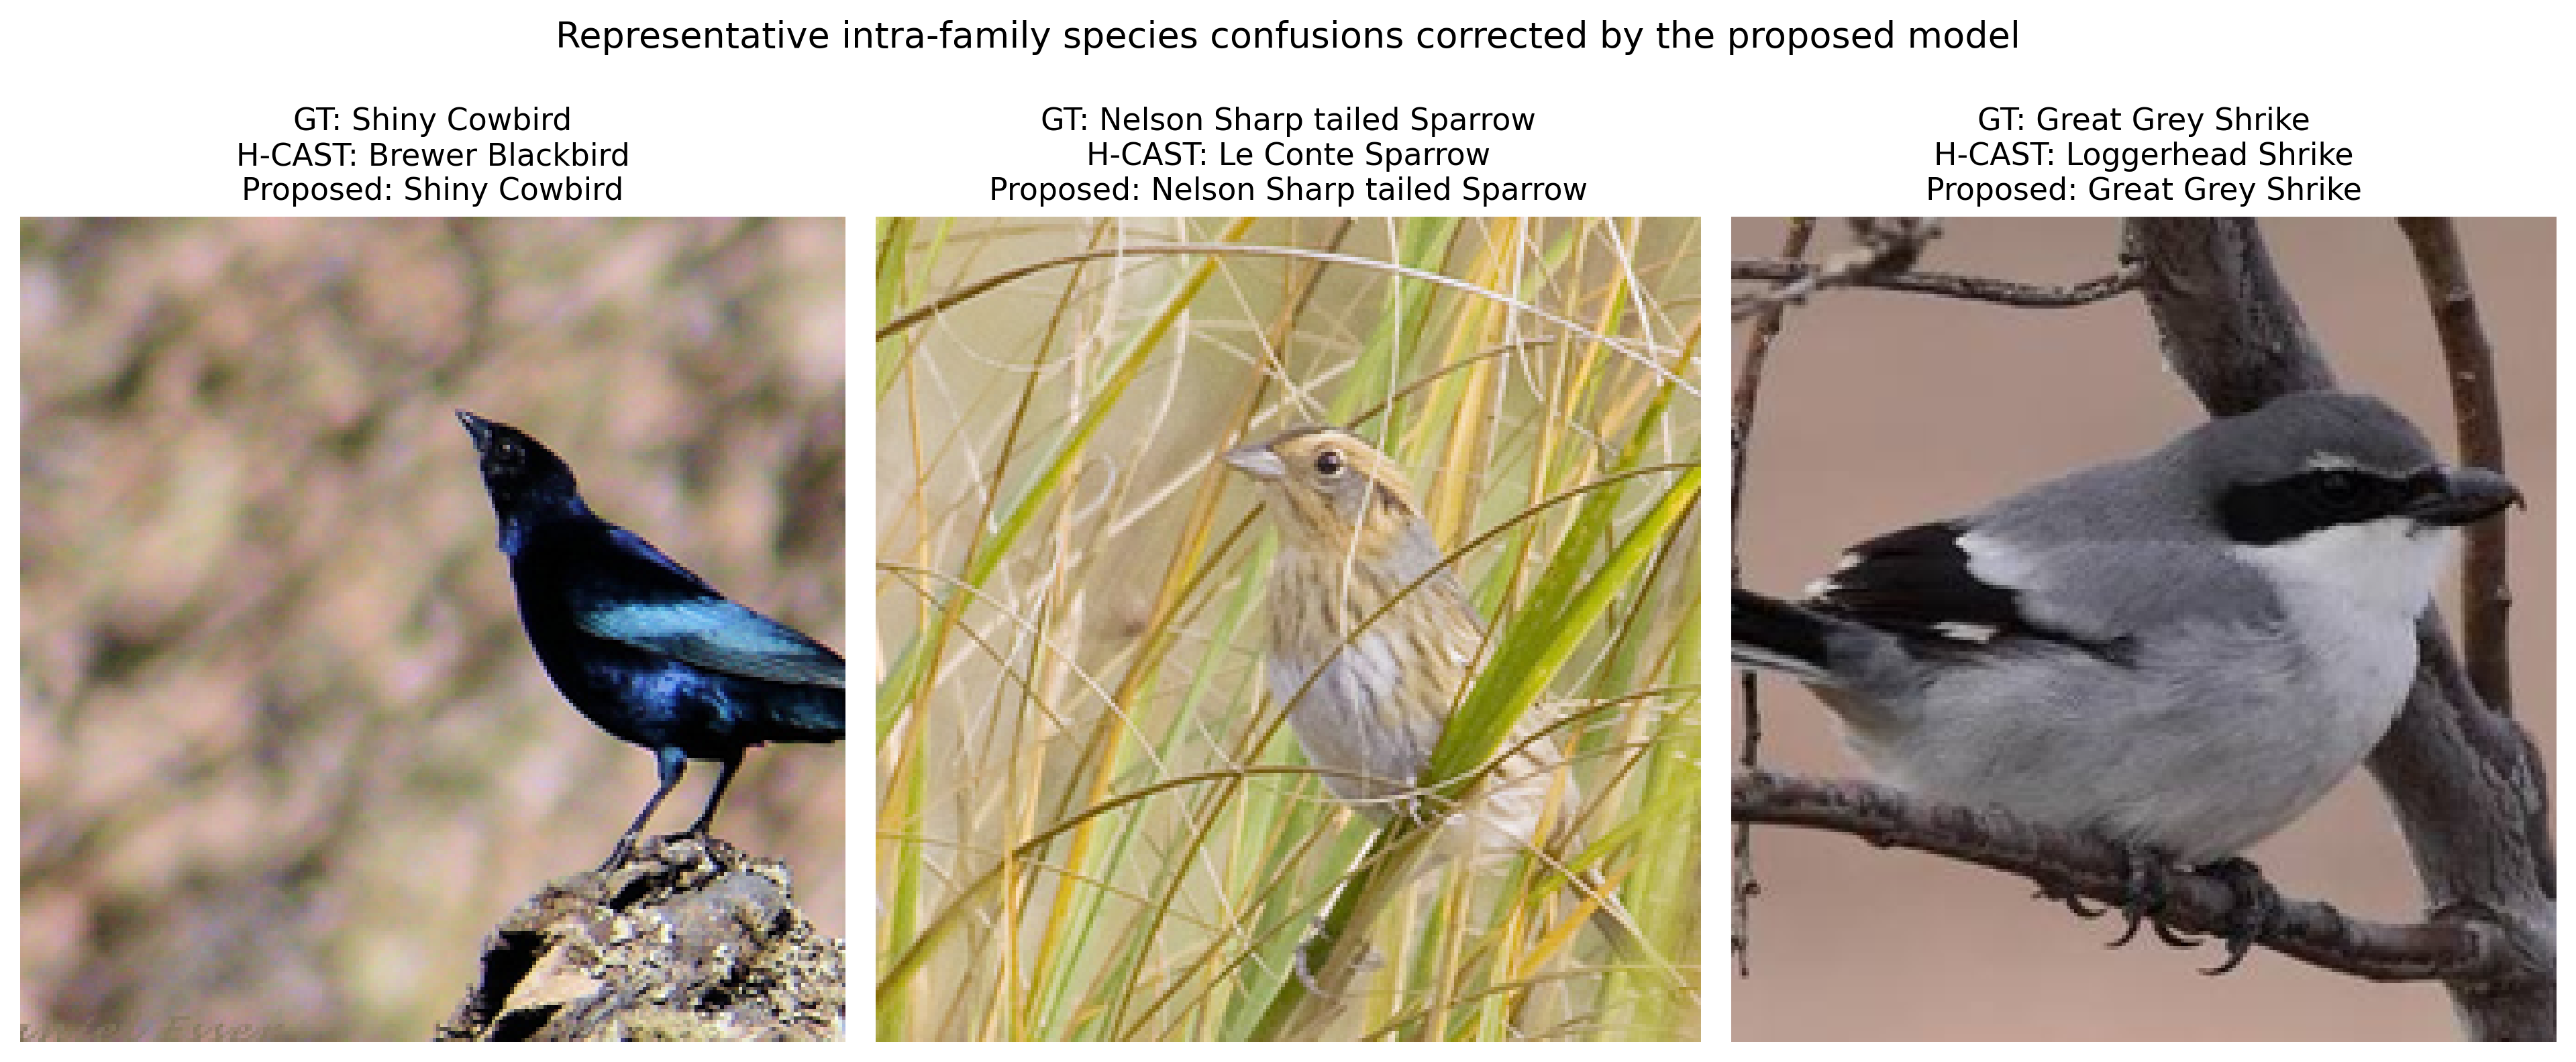
\includegraphics[width=\textwidth]{figures/case_B_examples_model_crop.png}
    \caption{Representative intra-family species confusions corrected by the proposed model. In each example, H-CAST predicts an incorrect species while still predicting the correct family, whereas the proposed attribute-guided model predicts the correct species.}
    \label{fig:case_b_examples}
\end{figure}

Figure~\ref{fig:case_b_examples} shows representative intra-family confusion cases corrected by the proposed model. These examples illustrate the type of errors captured by the second row of Table~\ref{tab:case_analysis_counts}: the image-only H-CAST baseline already predicts the correct family but fails to distinguish the correct species, while the proposed model makes the correct species-level prediction. This supports the quantitative observation that the proposed attribute-guided model is particularly useful for some fine-grained species confusions within the same family.

It should be noted that these examples are illustrative rather than exhaustive. The main evidence for the improvement comes from the prediction-level counts and the quantitative metrics reported in the previous sections.


\subsection{Diagnostic Analysis of Attribute Attention}

In addition to the prediction-level case analysis, we inspect the internal attention behavior of the proposed attribute-guided module. This analysis is intended to provide diagnostic insight into how the attribute branch behaves, rather than to prove that the model accurately localizes semantic attributes.

The proposed module produces two attention signals. First, during species-level fusion, the species class token attends to the attribute-group features through an attention-pooling operation. This produces a distribution over active attribute groups and indicates which groups contribute more strongly to the fused species representation. Second, each attribute-group query cross-attends to the species-level graph nodes generated by the H-CAST backbone. These graph-node attention weights are back-projected to the initial superpixels using the H-CAST graph assignment structure and are overlaid on the input image for visualization.

For the three-level CUB hierarchy used in this thesis, the attribute-group queries attend to the species-level graph representation. The visualized images correspond to the evaluation input after resizing and center cropping, which is the same input view used by the model during inference.

The attention ranking analysis shows that the species-token pooling attention is often dominated by global morphology groups, especially \textit{size} and \textit{shape}. In many inspected examples, these two groups receive substantially higher pooling weights than most other groups. This suggests that the fusion module assigns high importance to global morphology-oriented attribute features. However, these weights should not be interpreted as evidence that the model precisely localizes size or shape in the image. Instead, they indicate that the fused species representation may rely on global cues such as morphology, silhouette, scale, or contextual information.

This behavior is partly related to the selected HSDAS-199 mask. In this mask, the \textit{size} group contains only one retained attribute state, while the \textit{shape} group contains only two retained states. Therefore, these groups provide limited within-group attribute classification supervision, especially for the singleton \textit{size} group. Their queries can still receive gradients through the species-level fusion path, so high CLS pooling weights may reflect classification-useful latent features rather than precisely localized semantic attribute evidence.

Figure~\ref{fig:attention_diagnostic} shows a representative diagnostic visualization. The CLS pooling chart shows the species-token attention over attribute groups. In this example, the highest-weighted groups are \textit{size}, \textit{shape}, and \textit{back pattern}. Since the top-ranked groups are often dominated by global morphology groups, the spatial heatmaps in Figure~\ref{fig:attention_diagnostic}(b) are selected from local or part-related groups for diagnostic inspection. These maps allow us to examine whether some attribute queries attend to plausible bird regions. In some examples, local attribute-query maps overlap with the bird body or discriminative parts. However, this behavior is not sufficiently consistent to support a strong claim of semantic attribute localization.

\begin{figure}[t]
    \centering

    \begin{subfigure}{0.95\textwidth}
        \centering
        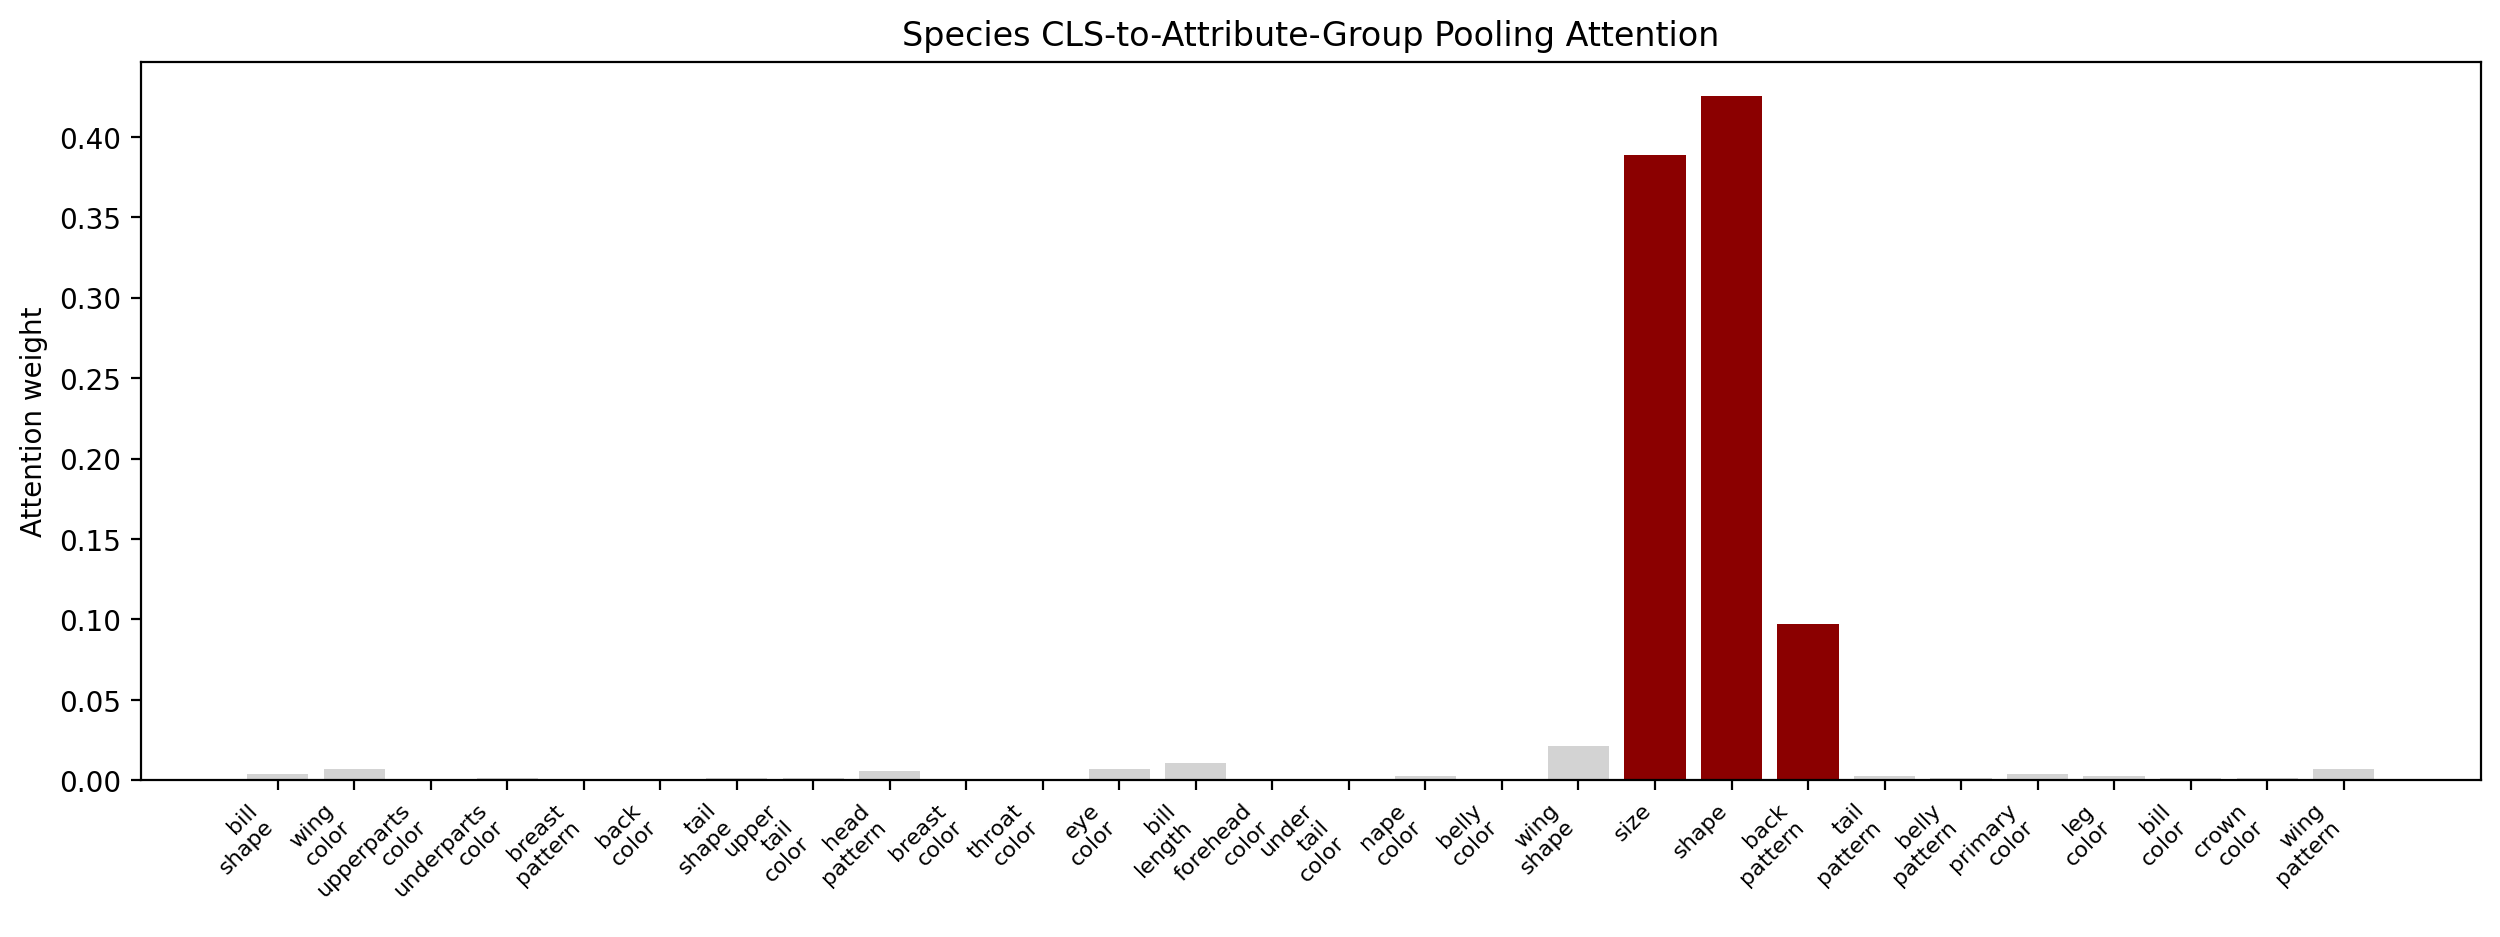
\includegraphics[width=\textwidth]{figures/case_California_Gull_0038_40865_cls_pooling.png}
        \caption{Species CLS-to-attribute-group pooling attention.}
        \label{fig:attention_diagnostic_cls}
    \end{subfigure}

    \vspace{0.5em}

    \begin{subfigure}{0.95\textwidth}
        \centering
        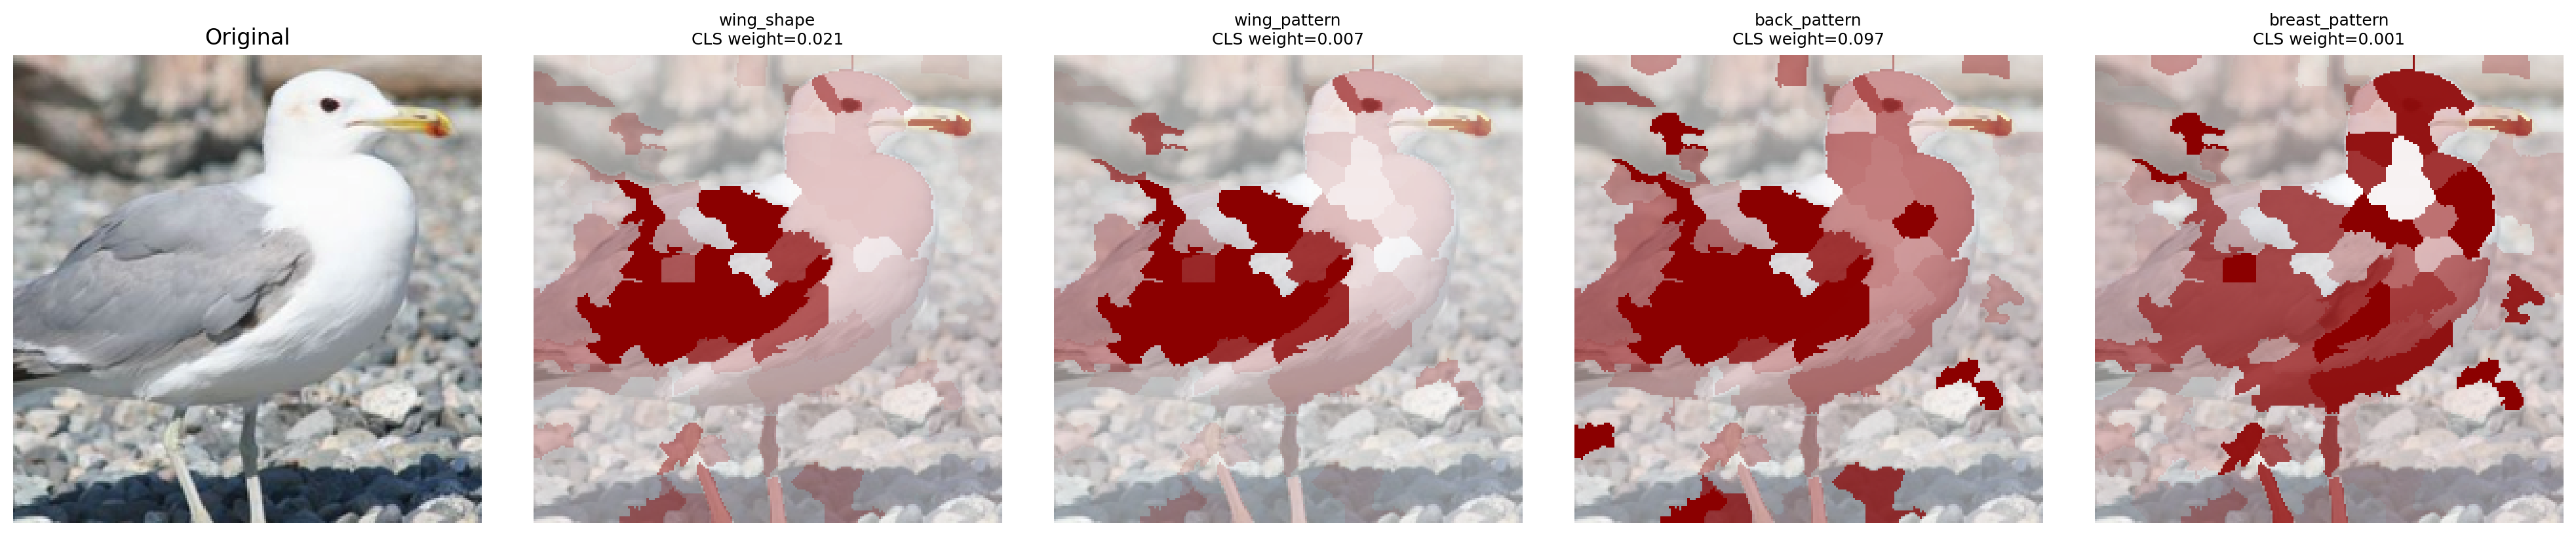
\includegraphics[width=\textwidth]{figures/case_California_Gull_0038_40865_attr_graph_top3_hard.png}
        \caption{Selected attribute-query spatial attention maps.}
        \label{fig:attention_diagnostic_spatial}
    \end{subfigure}

    \caption[Diagnostic visualization of the attribute-guided module.]
    {Diagnostic visualization of the attribute-guided module. 
    (a) The CLS pooling chart shows the species-token attention over attribute groups. In this example, the three highest-weighted groups are \textit{size}, \textit{shape}, and \textit{back pattern}, indicating that the fusion module assigns strong weight to global morphology-related groups. 
    (b) The spatial heatmaps show selected attribute-query attention maps back-projected to image superpixels. From left to right, the maps correspond to the original image, \textit{wing shape}, \textit{wing pattern}, \textit{back pattern}, and \textit{breast pattern}. These local or part-related groups are selected for diagnostic inspection and are not necessarily the highest-ranked groups in the CLS pooling distribution. These visualizations should not be interpreted as ground-truth attribute localization.}
    \label{fig:attention_diagnostic}
\end{figure}

The spatial attention maps of high-weight global groups further reveal a limitation of the current method. Although \textit{size} and \textit{shape} often receive high pooling weights, their graph-node attention maps are not consistently aligned with a clearly localized semantic part. In some inspected examples, these maps overlap with the bird body or head region, while in other cases they become diffuse or include substantial background regions. Therefore, high pooling weight for global morphology groups should not be interpreted as reliable evidence of precise attribute localization.

Figure~\ref{fig:size_shape_background_example} shows one representative limitation case. In this example, the \textit{size} and \textit{shape} attention maps place a substantial portion of their response on background regions instead of being tightly concentrated on the bird itself. This illustrates that even when these groups receive high CLS pooling weights, the corresponding spatial maps may still reflect a mixture of object cues, silhouette, scale, and contextual information rather than a precisely localized semantic attribute.

\begin{figure}[t]
    \centering
    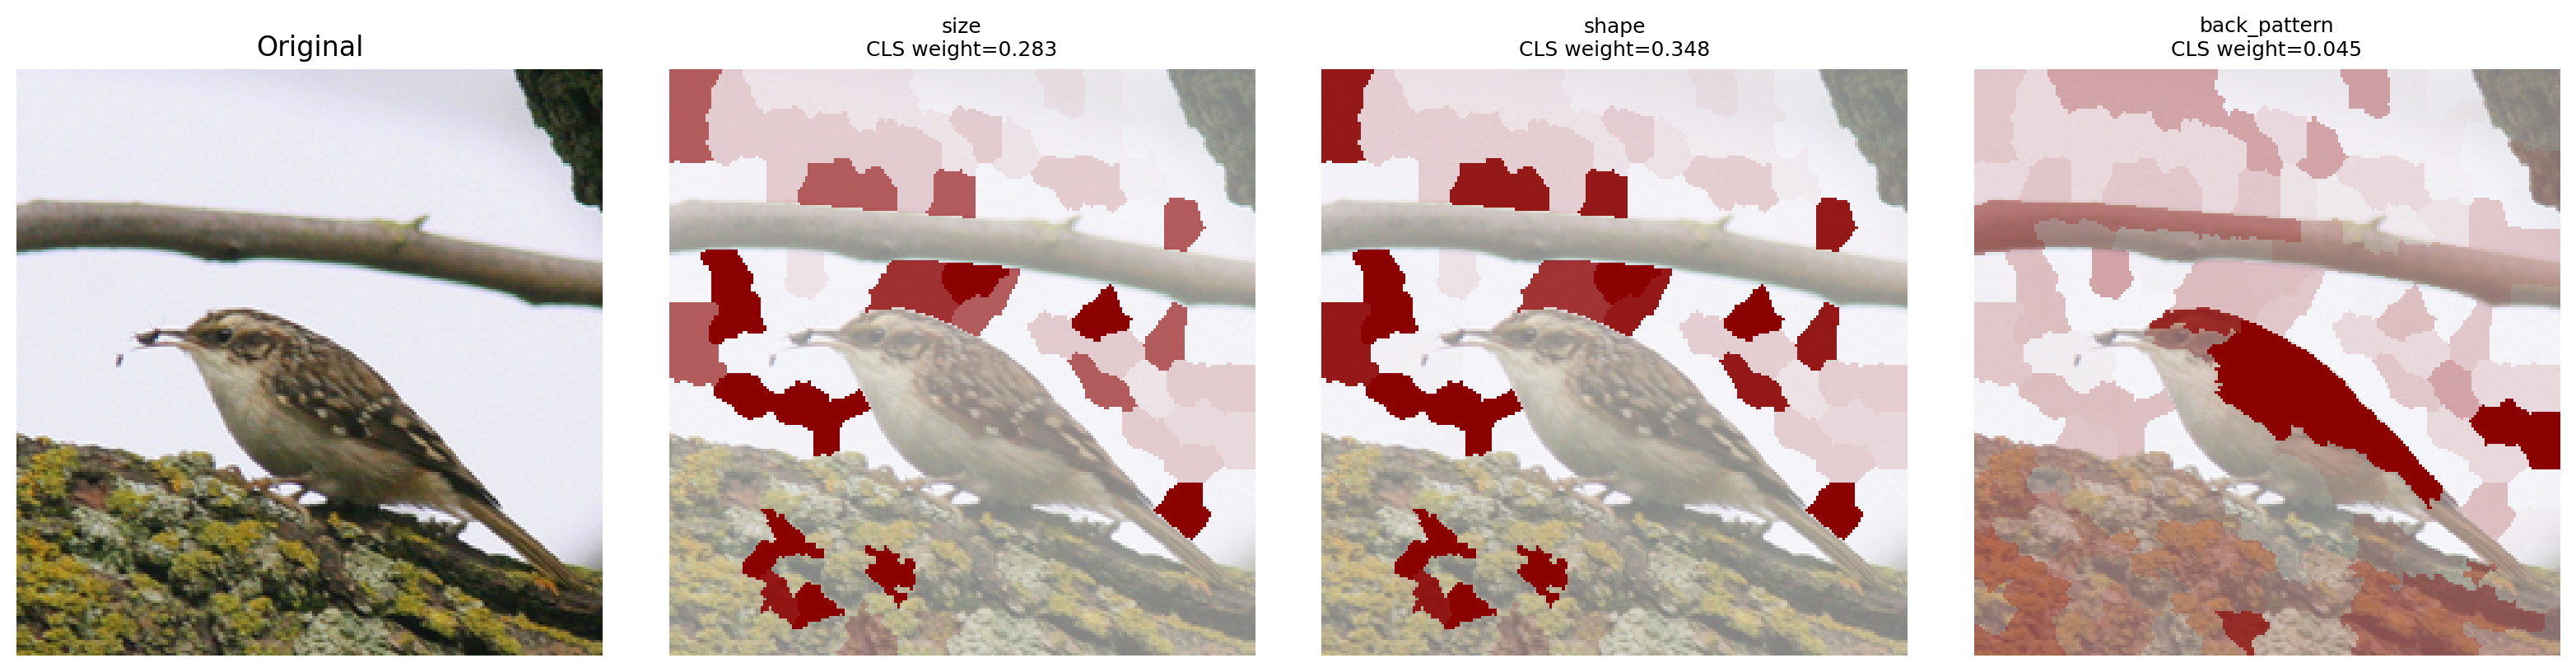
\includegraphics[width=0.92\textwidth]{figures/case_Brown_Creeper_0005_24659_attr_graph_top3_hard.png}
    \caption{Representative limitation case for high-weight global morphology groups. From left to right, the figure shows the original image, the spatial attention map of \textit{shape}, the spatial attention map of \textit{size}, and the spatial attention map of \textit{back pattern}. In this example, the \textit{shape} and \textit{size} queries place substantial attention on background regions. This indicates that these maps should be interpreted as diagnostic internal attention patterns rather than ground-truth localization of size or shape.}
    \label{fig:size_shape_background_example}
\end{figure}

For this reason, the attention visualizations are treated as diagnostic evidence rather than localization evidence. The model is trained with class-level attribute supervision and does not use pixel-level attribute localization labels. Therefore, it is not explicitly forced to align each attribute query with the corresponding semantic bird part. The main conclusion of this thesis is based on the quantitative results, ablation studies, and prediction-level case analysis, while the attention visualization is used only to better understand the internal behavior and limitations of the proposed module.


\subsection{Discussion}

The qualitative and diagnostic analyses provide a more detailed view of the quantitative results. The prediction-level case analysis shows that the proposed model corrects more species-level errors than it introduces. Specifically, it corrects 236 species-level errors made by the H-CAST rerun, while introducing 161 new species-level errors where H-CAST was originally correct. This results in a net gain of 75 correctly classified test images. Over 5,794 test images, this corresponds to approximately 1.29 percentage points, which is consistent with the observed species accuracy improvement from 84.55\% to 85.83\%.

The analysis also shows that many of the corrected cases are intra-family confusions. Among the 236 corrected species-level errors, 194 cases correspond to images where H-CAST predicts the correct family but the wrong species. This accounts for approximately 82.2\% of the corrected cases. This observation is consistent with the motivation of the proposed hard-sibling-aware attribute selection strategy, which is designed to prioritize attributes that help distinguish visually related species within the same family.

However, the proposed method is not uniformly better than the image-only H-CAST baseline. Some predictions that are correct in H-CAST become incorrect in the proposed model, and 659 images remain misclassified by both models at the species level. This indicates that attribute-guided fusion changes the species-level decision boundary and can improve average performance without improving every individual prediction. Therefore, the proposed method should be interpreted as improving species-level recognition overall, especially for some intra-family confusions, rather than as a model that consistently corrects all fine-grained errors.

The path-consistency analysis also helps explain the trade-off observed in the quantitative results. There are 86 images where the proposed model predicts the correct species but the full hierarchical path is still inconsistent. This is consistent with the fact that the proposed model achieves strong species accuracy, FPA, and wAP in the main setting, but does not obtain the lowest TICE among all ablation settings. Since attribute-guided fusion is applied mainly to the species-level branch, it can improve fine-grained species discrimination without necessarily improving taxonomy consistency in every case.

Finally, the attention analysis highlights an important limitation of the current approach. Although the attribute-guided branch improves classification performance, the attention visualizations do not provide strong evidence of precise semantic attribute localization. Global groups such as \textit{size} and \textit{shape} often dominate the pooling attention, and their spatial maps can be diffuse or include background regions. Some local attribute queries attend to plausible bird regions, but this behavior is not sufficiently consistent to support a strong localization claim. This suggests that the model may use a combination of object-part cues, global morphology, silhouette, scale, and contextual information.

Overall, the qualitative analysis supports the main conclusion of this thesis: attribute-guided fusion improves the main quantitative performance of H-CAST, especially species accuracy, FPA, and wAP, and many of the corrected errors are intra-family species confusions. At the same time, the diagnostic attention analysis shows that the current method should not be interpreted as a precise attribute localization model. Future work could address this limitation by incorporating object masks, part annotations, stronger localization constraints, or attention regularization methods that encourage attribute queries to focus more consistently on bird regions.